\chapter{Notes on backpropagation}\label{ch-07}

These notes contain the \textbf{complete derivation of the
backpropagation algorithm}, the algorithm that solves the \emph{credit
assignment} problem in multilayer networks introduced in
\href{06\%20-\%20Reti\%20neurali\%20(parte\%201)\%20-\%20dal\%20neurone\%20al\%20MLP}{06
- Neural networks (part 1) - from the neuron to the MLP}. The
professor insists on one point: \textbf{the derivation must be redone
by oneself, not memorised}. Only in this way is one able to recompute
it for different losses, activations or architectures --- and this is
the real goal. Implementing it in the project is the best way to
understand it thoroughly.

References: Rumelhart, Hinton, Williams, \emph{Parallel Distributed
Processing} (1986), ch.\ 8; Mitchell, \emph{Machine Learning}, ch.\ 4;
Haykin, \emph{Neural Networks}.

\section{Differential calculus
tools}\label{strumenti-di-calcolo-differenziale}

Gradient descent requires derivatives of composite functions. Three
rules are needed: \[
\frac{\partial f}{\partial x} = \frac{\partial f}{\partial g}\cdot\frac{\partial g}{\partial x} \quad \text{(chain rule)}, \qquad D[f(g(x))] = f'(g(x))\cdot g'(x), \qquad D[f\cdot g] = f'\cdot g + f\cdot g'.
\] The chain rule is useful because it \textbf{decomposes} the
computation, highlighting what can be computed immediately without
losing the general thread.

\section{The problem}\label{il-problema}

The basic architecture is a fully connected feedforward network (MLP).
Different indices are used for the layers: \(i\) for the input, \(j\)
for the hidden layer, \(k\) for the output.

\begin{figure}[htbp]
\centering
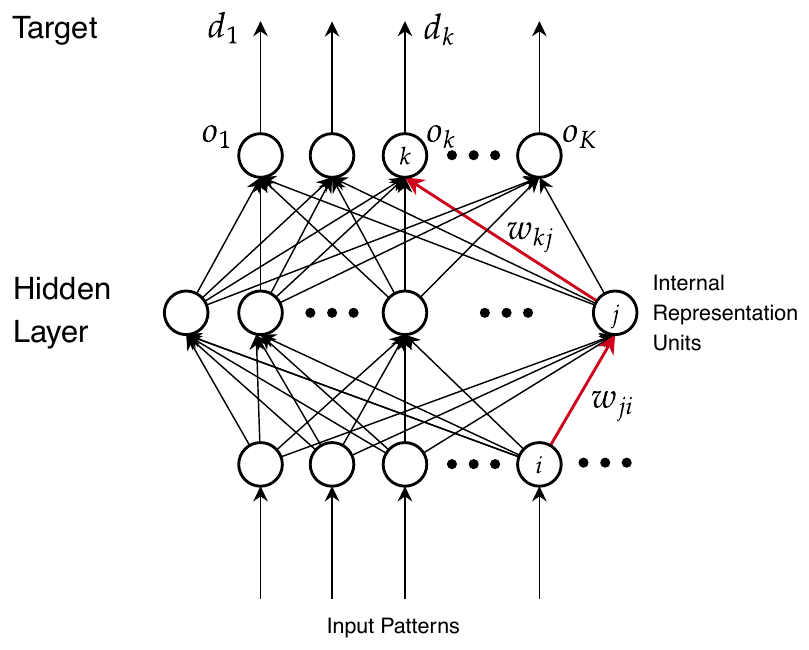
\includegraphics[width=0.54\linewidth,height=0.42\textheight,keepaspectratio]{images/07-bp_rete.png}
\caption{The reference network: input \(i\), hidden units \(j\), output
units \(k\).}
\end{figure}

\begin{boxdefinition}{The backpropagation problem}

Estimate the \textbf{contribution of the hidden units to the error} at
the output. This is done by computing the \textbf{Generalized Delta
Rule}.

\end{boxdefinition}

The training set is
\(TR = \{(\mathbf{x}^1, \mathbf{d}^1), \dots, (\mathbf{x}^l, \mathbf{d}^l)\}\)
(supervised learning). Each input unit \(i\) loads the component
\(x_i\) of the pattern: \(o_i = x_i\).

The \textbf{total error} of the network on the training set is \[
E_{tot} = \sum_p E_p, \qquad E_p = \frac{1}{2}\sum_{k=1}^{K}(d_k - o_k)^2,
\] where \(E_p\) is the error on pattern \(p\) computed over all \(K\)
output units. (The factor \(\frac{1}{2}\) only serves to simplify the
derivative.) To lighten the notation, from now on the index \(p\) is
omitted: \(o_k\) stands for \(o_k(\mathbf{x}_p)\) and \(d_k\) for
\(d_{p,k}\).

\textbf{Goal}: find the weights \(\mathbf{w}\) that minimise
\(E_{tot}\) (for now only the data term). It is still a least squares
minimisation (LMS). \textbf{Idea}: go down the surface of \(E_{tot}\)
following the gradient.

\begin{figure}[htbp]
\centering
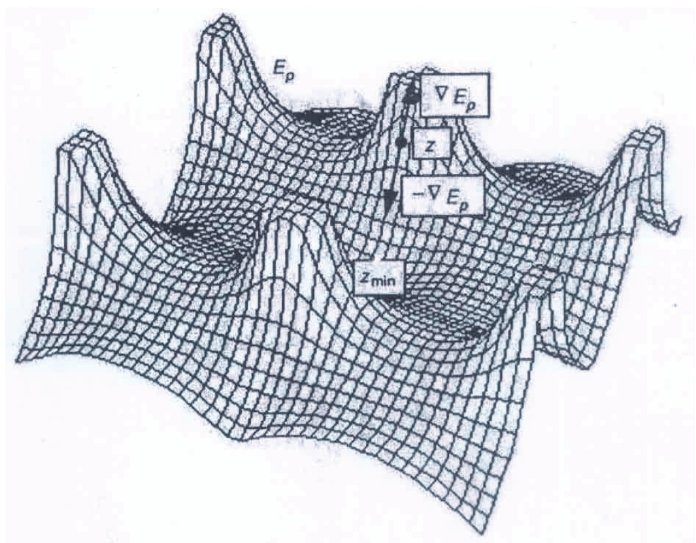
\includegraphics[width=0.54\linewidth,height=0.42\textheight,keepaspectratio]{images/07-bp_superficie.png}
\caption{A landscape of \(E_{tot}\) in the space of two weights:
following \(-\nabla E\) from point \(Z\) we reach \(Z_{min}\). Unlike
the linear model, the surface is not convex.}
\end{figure}

\section{The iterative algorithm}\label{lalgoritmo-iterativo}

The loss is computed, its gradient is computed, all weights are
updated; this is repeated until convergence or another stopping
criterion.

\begin{boxabstract}{Algorithm 1 --- Backpropagation}

Initialise all the weights \(\mathbf{w}\) of the network and \(\eta\).
Compute the outputs of the units and \(E_{tot}\). \textbf{While}
\(E_{tot} > \epsilon\) (or another criterion): - for each
\(w \in \mathbf{w}\):
\(\Delta w = -\dfrac{\partial E_{tot}}{\partial w}\) \textbf{(step 1)};
- \(w_{new} = w + \eta\,\Delta w + \dots\) \textbf{(step 2)}; -
recompute the outputs and \(E_{tot}\).

\end{boxabstract}

There are stochastic (on-line) and batch versions. Two aspects must be
distinguished:

\begin{enumerate}
\def\labelenumi{\arabic{enumi}.}
\tightlist
\item
  the \textbf{computation of the gradient} \(\partial E_{tot}/\partial w\),
  for each weight of the network: this is what backpropagation does;
\item
  the weight \textbf{update rule}: standard backprop, Quickprop,
  R-prop, \ldots{}
\end{enumerate}

We focus on step 1: \[
\Delta w = -\frac{\partial E_{tot}}{\partial w} = -\sum_p \frac{\partial E_p}{\partial w} \overset{def}{=} \sum_p \Delta_p w.
\]

\section{The derivation}\label{la-derivazione}

\subsection{The gradient for a generic
weight}\label{il-gradiente-per-un-peso-generico}

Consider a generic weight \(w_{tu}\), which connects the input coming
from a generic unit \(u\) (which can be \(i\) or \(j\)) to the generic
unit \(t\). Since \[
net_t = \sum_s w_{ts}\,o_s, \qquad o_t = f_t(net_t),
\] applying the chain rule through \(net_t\): \[
\Delta_p w_{tu} = -\frac{\partial E_p}{\partial w_{tu}} = \underbrace{-\frac{\partial E_p}{\partial net_t}}_{\delta_t}\cdot\underbrace{\frac{\partial net_t}{\partial w_{tu}}}_{o_u} = \delta_t\cdot o_u.
\] Indeed
\(\frac{\partial net_t}{\partial w_{tu}} = \frac{\partial \sum_s w_{ts} o_s}{\partial w_{tu}} = o_u\):
all terms of the sum are constant with respect to \(w_{tu}\) except the
one with \(s = u\). (The \(o_s\) are the inputs of unit \(t\).)

We have defined the \textbf{delta of unit \(t\)}: \[
\delta_t = -\frac{\partial E_p}{\partial net_t}.
\] Let us expand it further with the chain rule, going through
\(o_t = f_t(net_t)\): \[
\delta_t = -\frac{\partial E_p}{\partial net_t} = -\frac{\partial E_p}{\partial o_t}\cdot\frac{\partial o_t}{\partial net_t} = -\frac{\partial E_p}{\partial o_t}\cdot f'_t(net_t).
\] It remains to compute \(-\frac{\partial E_p}{\partial o_t}\), and
here two cases are distinguished: \(t\) is an \textbf{output unit}
\(k\), or a \textbf{hidden unit} \(j\).

\subsection{\texorpdfstring{Case 1: output unit
(\(t = k\))}{Case 1: output unit (t = k)}}\label{caso-1-unituxe0-di-uscita-t-k}

The output \(o_k\) appears directly in \(E_p\): \[
-\frac{\partial E_p}{\partial o_k} = -\frac{\partial\,\frac{1}{2}\sum_{r=1}^{K}(d_r - o_r)^2}{\partial o_k} = (d_k - o_k),
\] because only the term \(r = k\) depends on \(o_k\), and its
derivative is \(\frac{1}{2}\cdot 2(d_k - o_k)\cdot(-1)\). Hence: \[
\boxed{\delta_k = (d_k - o_k)\cdot f'_k(net_k)}
\] This is exactly the delta already seen for the single sigmoidal
unit: the error is directly measurable because we know the target.

\subsection{\texorpdfstring{Case 2: hidden unit
(\(t = j\))}{Case 2: hidden unit (t = j)}}\label{caso-2-unituxe0-nascosta-t-j}

For a hidden unit there is no target: \(o_j\) does not appear directly
in \(E_p\). However, \(o_j\) affects \(E_p\) \textbf{through all the
output units} it is connected to: each \(net_k\) depends on \(o_j\).
Applying the chain rule with a sum over all \(k\): \[
-\frac{\partial E_p}{\partial o_j} = \sum_{k=1}^{K}\underbrace{-\frac{\partial E_p}{\partial net_k}}_{\delta_k}\cdot\frac{\partial net_k}{\partial o_j} = \sum_{k=1}^{K}\delta_k\, w_{kj},
\] since
\(\frac{\partial net_k}{\partial o_j} = \frac{\partial \sum_s w_{ks}\,o_s}{\partial o_j} = w_{kj}\).
Hence: \[
\boxed{\delta_j = \left(\sum_{k=1}^{K}\delta_k\, w_{kj}\right)\cdot f'_j(net_j)}
\]

\begin{boxtip}{The crucial point}

The term \(-\frac{\partial E_p}{\partial net_k}\) \textbf{has already
been computed}: it is \(\delta_k\)! The delta of a hidden unit is thus
obtained by \textbf{propagating backwards} the deltas of the output
units, weighted by the same weights \(w_{kj}\) used in forward
propagation. Hence the name \textbf{back-propagation}: the error
``climbs back'' through the network. This solves credit assignment: the
``blame'' of a hidden unit is the sum of the blames of the units it
contributes to, weighted by how much it contributes.

\end{boxtip}

\begin{figure}[htbp]
\centering
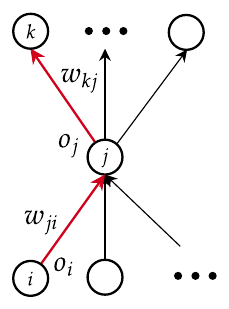
\includegraphics[width=0.21\linewidth,height=0.42\textheight,keepaspectratio]{images/07-bp_localita.png}
\caption{Using the network graph to localise the computation: each term
involves only adjacent units and weights.}
\end{figure}

Some remarks on case 2:

\begin{itemize}
\tightlist
\item
  it expresses the variation of \(E_p\) considering \textbf{all} the
  output units \(o_k\);
\item
  each \(o_k\) (and \(net_k\)) depends on \(o_j\): this is why the sum
  over \(k\) appears;
\item
  the same result can be obtained directly from the definition of
  \(E_p\) (as an exercise), but this form is more instructive because
  it shows the flow of partial derivatives \textbf{over the network}.
\end{itemize}

\section{Summary of the formulas}\label{sintesi-delle-formule}

For two layers we have derived: \[
\Delta_p w_{tu} = \delta_t\cdot o_u,
\] where \(\delta_t\) is the \textbf{error signal} available at unit
\(t\) and \(o_u\) is the input to \(t\) coming from \(u\) (through the
connection \(w_{tu}\)). In particular:

{\def\LTcaptype{none} % do not increment counter
\begin{longtable}[]{@{}
  >{\raggedright\arraybackslash}p{(\linewidth - 4\tabcolsep) * \real{0.3333}}
  >{\raggedright\arraybackslash}p{(\linewidth - 4\tabcolsep) * \real{0.3333}}
  >{\raggedright\arraybackslash}p{(\linewidth - 4\tabcolsep) * \real{0.3333}}@{}}
\toprule\noalign{}
\begin{minipage}[b]{\linewidth}\raggedright
Weight
\end{minipage} & \begin{minipage}[b]{\linewidth}\raggedright
Update
\end{minipage} & \begin{minipage}[b]{\linewidth}\raggedright
Delta
\end{minipage} \\
\midrule\noalign{}
\endhead
\bottomrule\noalign{}
\endlastfoot
\(w_{kj}\) (hidden → output) & \(\Delta_p w_{kj} = \delta_k\cdot o_j\)
& \(\delta_k = (d_k - o_k)\,f'_k(net_k)\) \\
\(w_{ji}\) (input → hidden) & \(\Delta_p w_{ji} = \delta_j\cdot o_i\)
& \(\delta_j = \left(\sum_{k}\delta_k\,w_{kj}\right) f'_j(net_j)\) \\
\end{longtable}
}

\begin{figure}[htbp]
\centering
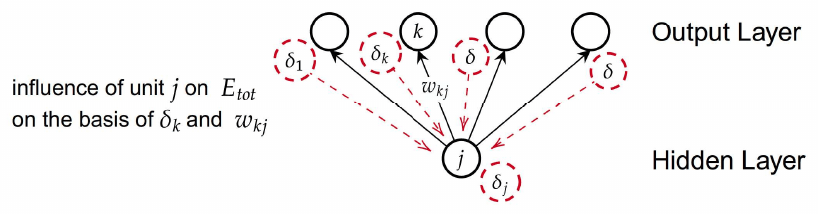
\includegraphics[width=0.71\linewidth,height=0.42\textheight,keepaspectratio]{images/07-bp_retropropagazione.png}
\caption{Backpropagation of the deltas: the influence of hidden unit \(j\)
on \(E_{tot}\) is computed from the \(\delta_k\) of the upper layer and
the weights \(w_{kj}\).}
\end{figure}

\subsection{\texorpdfstring{Generalisation to \(m\) hidden
layers}{Generalisation to m hidden layers}}\label{generalizzazione-a-m-strati-nascosti}

The derivation holds for \textbf{any number of hidden layers}: the
deltas do not come only from the output layer, but from any upper layer
\(h\) the unit is connected to. In general, \textbf{the deltas come
from all the units the current unit is connected to}: \[
\delta_j = \left(\sum_{h \in \text{successors}(j)}\delta_h\,w_{hj}\right) f'_j(net_j).
\] The update rule for each pattern (omitting \(p\)) is \[
w_{tu}^{new} = w_{tu} + \eta\,\delta_t\,o_u.
\] Using \(\Delta_p w\) for each pattern gives the \textbf{on-line}
version; for the \textbf{batch} version the contributions are summed
over all patterns before updating.

\section{The complete training
cycle}\label{il-ciclo-di-addestramento-completo}

\begin{enumerate}
\def\labelenumi{\arabic{enumi}.}
\tightlist
\item
  \textbf{Forward computation}: outputs of all units, layer by layer.
\item
  Computation of the \textbf{errors and deltas in the output layer}.
\item
  \textbf{Backward propagation} of the deltas from the output layer to
  the hidden layers.
\item
  \textbf{Weight update}.
\item
  Start again, until the stopping criterion.
\end{enumerate}

\begin{boxwarning}{Do not forget the biases}

Computation and update must also be applied to the \textbf{biases} of
all units: the first component of the input of each unit is assumed to
be 1, with the bias as weight \(w_{t0}\). Hence
\(\Delta w_{t0} = \delta_t \cdot 1\).

\end{boxwarning}

\section{Properties and
interpretation}\label{proprietuxe0-e-interpretazione}

\begin{itemize}
\tightlist
\item
  \textbf{Only local computations}: each unit directly uses only nearby
  information (the units below and above), not distant layers; the rest
  arrives indirectly through the flow of deltas. In other words: even
  though the computation is local, changing a weight has a
  \textbf{global effect} on the network. What is the influence of each
  \(w_{tu}\) on the global error? This complex effect has been
  \textbf{decomposed} into simple components through the deltas local
  to each unit.
\item
  \textbf{View as a diffusion process}: backpropagation is a local
  spatio-temporal propagation from the ``parents'' of the unit to the
  unit and from the unit to its ``children''.
\item
  \textbf{Efficiency --- the ``magic factorisation''}: the delta
  \(\delta_t\) of each unit is computed \textbf{only once} and reused
  for \textbf{all} its weights \(w_{tu}\). The cost is therefore
  proportional to the \textbf{number of weights}, not to its square.
  With models of billions of weights the difference is enormous:
  \(10^9\) versus \((10^9)^2 = 10^{18}\) operations, which would be
  infeasible.
\end{itemize}

\begin{boxtip}{Three levels of reading of the derivation}

\begin{enumerate}
\def\labelenumi{\arabic{enumi}.}
\tightlist
\item
  The individual \textbf{mathematical steps}.
\item
  The \textbf{interpretation} of the local variations of one quantity
  with respect to the others (the meaning of the partial derivatives).
\item
  The \textbf{big picture}: the decomposition serves to find the delta
  values of each level, decomposing the error \textbf{over the network}
  at hand.
\end{enumerate}

\end{boxtip}

\begin{boxwarning}{Correct terminology}

One does not say ``backprop network'': the neural network is the
\textbf{model}. Backpropagation is a \textbf{training algorithm} based
on the backward propagation of errors, i.e.\ on the direct computation
of the gradient through the network.

\end{boxwarning}

\begin{boxexample}{Numerical example (to check understanding)}

Network with one input \(x = 1\), one sigmoidal hidden unit and one
linear output unit, no bias; weights \(w_{ji} = 0.5\), \(w_{kj} = 1\),
target \(d = 1\), \(\eta = 0.1\). - Forward: \(net_j = 0.5\),
\(o_j = \sigma(0.5) \approx 0.622\);
\(o_k = 1 \cdot 0.622 = 0.622\). - Output delta (linear,
\(f' = 1\)): \(\delta_k = (1 - 0.622)\cdot 1 = 0.378\). - Hidden
delta:
\(\delta_j = (\delta_k w_{kj})\,\sigma'(net_j) = 0.378 \cdot 0.622 \cdot (1 - 0.622) \approx 0.089\).
- Updates:
\(\Delta w_{kj} = \eta\,\delta_k\,o_j \approx 0.1 \cdot 0.378 \cdot 0.622 \approx 0.0235\);
\(\Delta w_{ji} = \eta\,\delta_j\,x \approx 0.0089\).

Both weights increase, making the output grow towards the target.

\end{boxexample}

\begin{boxquestion}{Possible exam questions}

\begin{itemize}
\tightlist
\item
  Derive backpropagation for a two-layer MLP with squared error.
\item
  What is \(\delta_t\)? How is it computed for an output unit and for
  a hidden unit?
\item
  Why does backpropagation have a cost linear in the number of
  weights?
\item
  How does the derivation change with a different loss or with more
  hidden layers?
\end{itemize}

\end{boxquestion}
